\section{Esempio: Studio del Moto}

\subsection{Titolo e Scopo dell'Esperienza}
\textbf{Titolo:} Studio del Moto Uniformemente Accelerato\\
\textbf{Scopo:} Verificare sperimentalmente le leggi del moto uniformemente accelerato.

\subsection{Materiali e Strumenti}
\begin{itemize}
    \item Piano inclinato (base \SI{2000}{\milli\metre}) e inclinato di \SI{30}{\degree}.
    \item Sfera metallica.
    \item Cronometro digitale (sensibilità: \SI{0,01}{\second}, portata: \SI{999,99}{\second}).
    \item Metro a nastro (sensibilità: \SI{1}{\milli\metre}, portata: \SI{3000}{\milli\metre}).
    \item Goniometro (sensibilità: \SI{1}{\degree}, portata: \SI{180}{\degree}).
\end{itemize}

\begin{figure}[!htbp] 
    \centering
    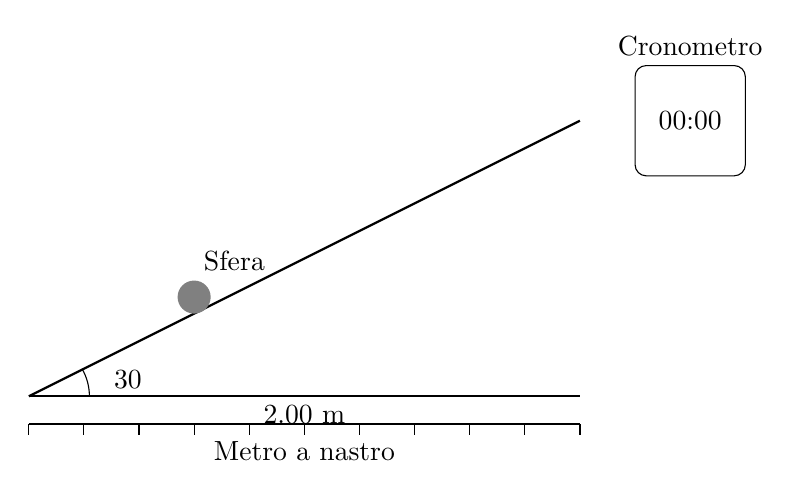
\begin{tikzpicture}[scale=0.7]
        % Piano inclinato
        \draw[thick] (0,0) -- (10,5);
        \draw[thick] (0,0) -- (10,0);
        
        % Sfera
        \fill[gray] (3,1.8) circle (0.3);
        
        % Cronometro
        \draw[rounded corners] (11,4) rectangle (13,6);
        \node at (12,5) {00:00};
        
        % Metro a nastro
        \draw[thick] (0,-0.5) -- (10,-0.5);
        \foreach \x in {0,1,...,10}
            \draw (\x,-0.7) -- (\x,-0.5);
        \node at (5,-1) {Metro a nastro};
        
        % Goniometro
        \draw (1.1,0) arc (0:30:1);
        \node at (1.8,0.3) {$\SI{30}{\celsius}$};
        
        % Etichette
        \node[below] at (5,0) {2.00 m};
        \node[above right] at (3,2.1) {Sfera};
        \node[above] at (12,6) {Cronometro};
    \end{tikzpicture}
    \caption{Apparato sperimentale per lo studio del moto uniformemente accelerato.}
    \label{fig:apparato}
\end{figure}

\subsection{Raccolta Dati}
Abbiamo misurato il tempo impiegato dalla sfera per percorrere diverse distanze lungo il piano inclinato, inclinato di \SI{30}{\degree} rispetto all'orizzontale.

\begin{table}[!htbp] 
    \centering
    \begin{tabular}{@{}ccc@{}}
        \toprule
        Distanza (\si{\metre}) & Tempo (\si{\second}) & Errore sul tempo (\si{\second}) \\
        \midrule
        0,200 & 0.29 & 0,01 \\
        0,400 & 0.41 & 0,01 \\
        0,600 & 0.50 & 0,01 \\
        0,800 & 0.58 & 0,01 \\
        1,000 & 0.65 & 0,01 \\
        \bottomrule
    \end{tabular}
    \caption{Dati sperimentali}
    \label{tab:datitab}
\end{table}

\subsection{Cenni Teorici}
Nel moto uniformemente accelerato, la posizione $s$ in funzione del tempo $t$ è data da:

\begin{equation}
    s = \frac{1}{2}at^2
\end{equation}

dove $a$ è l'accelerazione. Nel nostro caso, l'accelerazione lungo il piano inclinato è data da:

\begin{equation}
    a = g\sin\theta
\end{equation}

dove $g$ è l'accelerazione di gravità e $\theta$ è l'angolo di inclinazione del piano.

\subsection{Elaborazione Dati}
Per verificare la relazione $s = \frac{1}{2}at^2$, plotteremo $s$ in funzione di $t^2$. La pendenza della retta di best fit sarà $\frac{1}{2}a$.

\subsection{Calcolo degli Errori nelle Misure Indirette}
L'errore su $t^2$ si propaga come:

\begin{equation}
    \Delta(t^2) =\overline{t^2} \left(2\cdot\frac{\Delta t}{\overline{t}}  \right)= 2\overline{t}\Delta t.
\end{equation}
Con questa formula, calcoliamo gli errori su $t^2$ e li mettiamo in tabella:

\begin{table}[h!]
\centering
\begin{tabular}{|c|c|}
\hline
$t^2$ (\si{\square\s}) & $\Delta \left( t^2 \right)$ (\si{\square\s}) \\
\hline
0.0841 & 0.006 \\
0.1681 & 0.008 \\
0.25   & 0.01   \\
0.3364 & 0.01 \\
0.4225 & 0.01  \\
\hline
\end{tabular}
\caption{Valori calcolati di $t^2$ e $\Delta t^2$}
\end{table}

\subsection{Grafico Sperimentale}

\begin{figure}[!htbp] 
    \centering
    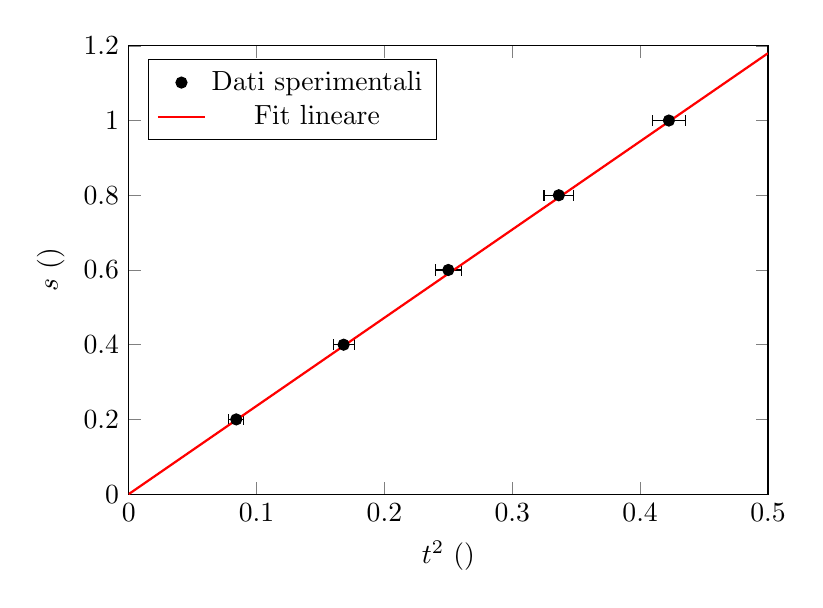
\begin{tikzpicture}
        \begin{axis}[
            width=0.8\textwidth,
            height=0.6\textwidth,
            xlabel={$t^2$ (\si{\second\squared})},
            ylabel={$s$ (\si{\metre})},
            xmin=0, xmax=0.5,
            ymin=0, ymax=1.2,
            legend pos=north west,
            ]
            \addplot[only marks,error bars/.cd,x dir=both,x explicit,y dir=both,y explicit]
            coordinates {
                (0.0841, 0.20) +- (0.0058, 0.001)
                (0.1681, 0.40) +- (0.0082, 0.001)
                (0.2500, 0.60) +- (0.0100, 0.001)
                (0.3364, 0.80) +- (0.0116, 0.001)
                (0.4225, 1.00) +- (0.0130, 0.001)
            };
            \addplot[domain=0:0.5, samples=100, smooth, thick, red] {2.3604*x};
            \legend{Dati sperimentali, Fit lineare}
        \end{axis}
    \end{tikzpicture}
    \caption{Grafico di $s$ in funzione di $t^2$.}
    \label{fig:grafico}
\end{figure}
Il grafico con le barre di errore è stato ottenuto con un software perché non è possibile realizzarlo coi fogli google (non si possono inserire barre di errore personalizzate ad esempio). Ovviamente si può realizzare un ottimo grafico manuale con le tecniche esposte nei precedenti paragrafi.
\subsection{Conclusioni}
Dal fit lineare dei dati, abbiamo ottenuto una pendenza di \SI{2.3604}{\metre\per\second\squared}, che corrisponde a $\frac{1}{2}a$. La pendenza si misura sul grafico tracciando la retta a mano  oppure, se si è realizzato il grafico col foglio di calcolo, basta fargli scrivere l'equazione che sarà del tipo $y= bx +a$, dove $b$ è la pendenza. Quindi, l'accelerazione sperimentale è:

\begin{equation}
    a_{\text{exp}} = \SI{4.7208}{\metre\per\second\squared}
\end{equation}

Teoricamente, l'accelerazione dovrebbe essere:

\begin{equation}
    a_{\text{th}} = g\sin\theta = \SI{9.81}{\metre\per\second\squared} \cdot \sin(\SI{30}{\degree}) = \SI{4.905}{\metre\per\second\squared}
\end{equation}

La differenza relativa tra il valore sperimentale e quello teorico è:

\begin{equation}
    \frac{|a_{\text{exp}} - a_{\text{th}}|}{a_{\text{th}}} \cdot 100\% = \frac{|\SI{4.7208}{\metre\per\second\squared} - \SI{4.905}{\metre\per\second\squared}|}{\SI{4.905}{\metre\per\second\squared}} \cdot 100\% \approx 3.75\%
\end{equation}

Notiamo che non abbiamo potuto fare il confronto col metodo degli errori (sezione 2.4) perché non abbiamo calcolato l'errore sull'accelerazione e sul valore teorico atteso (sarebbe stato troppo complicato). Comunque, questa discrepanza del 3.75 \% tra il valore sperimentale e quello teorico è accettabile per un esperimento di laboratorio di fisica elementare. Le possibili fonti di errore includono:

\begin{itemize}
    \item Piccoli errori nella misurazione del tempo.
    \item Leggero attrito tra la sfera e il piano inclinato.
    \item Possibile imprecisione nella misurazione dell'angolo di inclinazione.
    \item Errori di parallasse nella lettura delle distanze.
\end{itemize}

Per migliorare ulteriormente l'esperimento, si potrebbe:
\begin{itemize}
    \item Utilizzare un sistema di rilevamento del tempo più preciso, come un timer fotoelettrico.
    \item Ridurre l'attrito utilizzando una superficie più liscia o una sfera con minore attrito.
    \item Ripetere le misurazioni più volte per ogni distanza per ridurre gli errori casuali.
\end{itemize}

In conclusione, l'esperimento ha confermato con buona approssimazione la relazione tra spazio e tempo nel moto uniformemente accelerato, dimostrando l'efficacia del metodo sperimentale nell'investigare le leggi della fisica.

\chapter{Guida linguaggio python}



